\chapter{A comprehensive heavy-flavor dynamical modeling framework}
\label{chapter:coupling}
The dynamical modeling framework for heavy flavor particles is summarized in the flow chart in figure \ref{fig:flowchart}.
The soft initial condition model provides both the initial energy density of the medium and the location of the hard particle production vertices in the transverse plane, while pQCD based calculations provide the momentum space distribution of the hard partons.
The left branch of this flow chart -- the hydrodynamic-based medium evolution model -- has been discussed in chapter \ref{chapter:simulation}.
We briefly review the RHS of the flow chart -- the multi-stage model for heavy-flavor evolution.
The hard production model is introduced in section \ref{section:hard}.
The initially produced partons are highly virtual and undergo the scale evolution that bring down the virtuality; eventually, at some point, this evolution will be matched to the in-medium transport calculations.
There is a complication regarding vacuum-like parton showers in a medium since certain vacuum parton branchings occupy the same space-time volume as the medium and also receive medium corrections.
Another obstacle is that multiple emissions are treated very differently between vacuum-like showers and medium-induce showers.
For the vacuum evolution, the ``time'' variable is the virtuality scale with the space-time information integrated out, while the transport model evolves the systems in real-time, with virtuality integrated out below a specific in-medium scale.
Significant progress has been made in both theory and design of event-generators to solve this problem \cite{MehtarTani:2012cy,Mehtar-Tani:2017ypq,Cao:2017zih,Kauder:2018cdt,Putschke:2019yrg,PhysRevLett.120.232001,Caucal:2018ofz}.
In section \ref{section:match}, we discuss a possible prescription to interface the two types of showers in our simulation.
Section \ref{section:couple-to-hydro} contains details of coupling the transport model to a dynamically evolving medium with large longitudinal expansion.
The heavy flavor hadronization model and hadronic rescatterings are introduced in section \ref{section:hadronization}.
The hadronization routine applies a previously used implementation \cite{Cao:2013ita} of the high-$p_T$ fragmentation plus low-$p_T$ recombination model for heavy hadrons production \cite{Oh:2009zj}.
Finally, in section \ref{section:benchmark}, the model is benchmarked using a few values of fixed coupling constant and running coupling constants, before being systematically calibrated to data in the next chapter.

\begin{figure}
\singlespacing
\centering
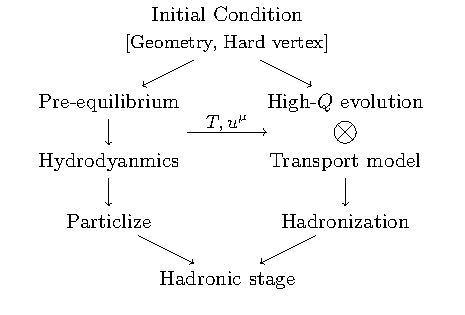
\includegraphics[width=.8\textwidth]{flowchart.pdf}
\caption[A schematic workflow of the heavy quark simulation. The left]{A schematic workflow of the heavy quark simulation. The left branch evolves the medium in the hydrodynamic based model, providing medium information (temperature, flow velocity) to the hard probe transport in the right branch. The hard and soft hadrons are evolved in the hadronic afterburner in the last step.}
\label{fig:flowchart}
\end{figure}

\section{Initial production of heavy flavor}
\label{section:hard}
\subsection{Factorization framework in proton-proton collisions}
In the proton-proton collision, hard processes can be computed in the factorization framework using pQCD-based techniques as schematically demonstrated in \ref{fig:factorization}.
The incoming proton is a composite object and there is a certain ``probability'' of finding a parton $i(j)$ carrying $x_i(x_j)$ fraction of the momentum of the proton $p_1(p_2)$.
This ``probability'' is known as the parton distribution function (PDF) $f_i(x, Q^2)$.
It not only is a function of $x$, but also depends on the scale $Q^2$ at which the proton is probed.
The probing scale is required to be much larger than the non-perturbative scale $Q^2 \gg \Lambda^2$ such that $\alpha_s(Q^2)$ is small due to asymptotic freedom, and the process of partons $i$ and $j$ scattering into partons $k$ and $l$ is perturbatively computable.
The partonic final state eventually hadronizes via non-perturbative processes.
The parton fragmentation function is defined as the probability to find a certain hadron $H$ carrying a fraction $x_H$ of the parton's momentum.
Combing these pieces together, the cross-section for the inclusive production of the hadron $H$ can be written as \cite{Field:1989uq},
\begin{eqnarray}
\frac{d\sigma_{p+p\rightarrow H+X}}{dy d\mathbf{p}_T^2} = \frac{1}{\pi}\int dx_i dx_j f_i(x_i, Q^2) f_j(x_j, Q^2) \frac{d\sigma_{ij\rightarrow kl}}{d\hat{t}} \frac{1}{z_k}D^H(z_k, Q^2).
\end{eqnarray}
Although the parton distribution function $f$ and the parton fragmentation function $D$ are essentially non-perturbative objects, they parametrize universal long-distance physics and can be extracted from independent experiments at certain scales $Q_0^2$.
Moreover, the evolution from the ``definition'' scale $Q_0^2$ to the process scale $Q^2$ can be described by the Dokshitzer-Gribov-Lipatov-Altarelli-Parisi (DGLAP) evolution equations \cite{Gribov:1972ri,Altarelli:1977zs,Dokshitzer:1977sg} based on pQCD to increase the predictive power of the calculation.

\begin{figure}
\singlespacing
\centering
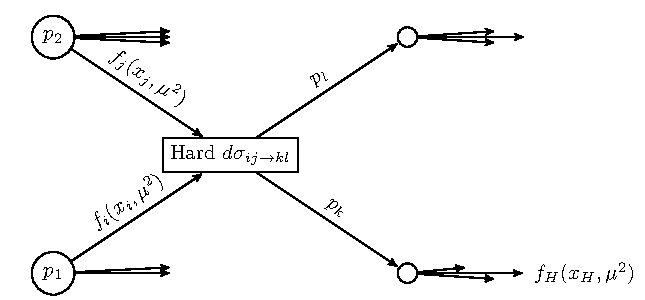
\includegraphics[width=.8\textwidth]{factorization.pdf}
\caption[A schematic demonstration of the factorization theorem. The]{A schematic demonstration of the factorization theorem. The momenta of the two incoming protons are $p_1$ and $p_2$. $f_{i,j}$ are the parton distribution function. $d\sigma$ is the perturbative matrix-element. $f_H$ is the fragmentation function.}
\label{fig:factorization}
\end{figure}

\subsection{The DGLAP evolution equation and the vacuum parton shower} The DGLAP evolution takes into account that the initial high-virtuality parton $i$ (or $j$) could have come from a splitting process of a parton with lower virtuality parton $i'$ (or $j'$).
Similarly, the final state high virtuality parton $k$ (or $l$) could also split into a low virtuality parton $k'$ (or $l'$) before it turns into a hadron.
Though each splitting causes an additional power of $\alpha_s$, it is also magnified by a potentially large factor $\ln (Q^2/\mu^2)$ when $Q^2$ is much higher than the scale where the $f$, $D$ are defined.
The same argument also applies to partons $i', j', k', l'$. 
The DGLAP equations systematically resum contributions including an arbitrary number of parton splittings and evolve the scale from $\mu^2$ to the hard scale $Q^2$.
Take the evolution equation for quark distribution function as an example,
\begin{eqnarray}
\frac{\partial f_q(x, Q^2)}{\partial \ln Q^2} &=& \frac{\alpha_s C_F}{2\pi} \int_x^1 \frac{dz}{z} \left(\frac{1+z^2}{(1-z)_+} + \frac{3}{2}\delta(1-z) \right)  f_q\left(\frac{x}{z}, Q^2\right)\\\nonumber
&&+ \frac{\alpha_s}{2\pi} \int_x^1 \frac{dz}{z} \frac{z^2+(1-z)^2}{2}f_g\left(\frac{x}{z}, Q^2\right).
\end{eqnarray}
where $x$ is the momentum fraction carried by the parton. The ``+'' subscript on a function defines the operation,
\begin{eqnarray}
\int_0^1 \frac{f(x)}{(1-x)_+} = \int_0^1 dx \frac{f(x)-f(1)}{1-x}.
\end{eqnarray}
Using
\begin{eqnarray}
\int_0^1 dx \frac{1+x^2}{(1-x)_+} = -\frac{3}{2}, P_{qg}^{q(0)}(z) = C_F\frac{1+z^2}{1-z}, P_{q\bar{q}}^{g(0)}(z) = \frac{z^2+(1-z)^2}{2}, 
\end{eqnarray}
The equation can be cast into a form similar to the transport equation,
\begin{eqnarray}
\frac{\partial f_q(x, Q^2)}{\partial \tau} &=&  \int_x^1 \frac{dz}{z}\left\{ P_{qg}^{q(0)}(z) f_q\left(\frac{x}{z}, Q^2\right) 
+ P_{q\bar{q}}^{g(0)}(z) f_g\left(\frac{x}{z}, Q^2\right)\right\} \\\nonumber&& - f_q\left(x, Q^2\right) \int_0^1 dz P_{qg}^{q(0)}(z).
\end{eqnarray}
where $\tau = \alpha_s/2\pi \ln Q^2$ plays the role of a ``time'', and the right-hand side contains the gain-term (feeding from quark and gluon splittings) and loss-term (splitting of a quark).
This probabilistic interpretation is beneficial for building a phenomenological parton-shower picture: 
each hard parton has certain probabilities to splits into two or more partons within a ``time'' interval from $\tau$ to $\tau+\Delta \tau$.
The newly created partons can also split in the next ``time'' step.
In this way, one can mimic the production of the exclusive partonic final state from the sequence parton branchings using Monte Carlo techniques.

\subsection{Production in the nuclear environment}
The above framework explains very well the hard production process in proton-proton collisions.
In a nuclear environment, there are several differences.
First, the parton distribution functions inside a nucleus differ from a simple superposition of the nucleon PDFs.
The ratio between the nuclear PDF and proton PDF generally deviates from unity.
In particular, this ratio for small $x$ gluons is significantly below one, known as the ``nuclear shadowing'' effect. 
This ratio increases and becomes larger than one at larger $x$, termed as the ``anti-shadowing'' region.
The difference between the nuclear PDF and proton PDF belongs to the category of ``cold nuclear matter'' (CNM) effect, in contrary to the ``hot nuclear matter'' effect from the QGP medium.
The CNM effect has to be included to correctly interpret the experimental data, though the current level of uncertainty on the nuclear PDF is still significant.

\subsection{Inclusive calculation versus Monte-Carlo event generator}
In the course of my study, I have tried using both an inclusive cross-section calculation as well as a Monte-Carlo event generator to initialize the heavy quark production.
The inclusive calculation directly applies the factorization theorem and computes the inclusive spectra of heavy quark/hadron production spectrum; while the event generator used the probabilistic picture of the DGLAP evolution to build an exclusive final state.

\paragraph{Initialization from an inclusive calculation of heavy flavor production}
We use a  FONLL (Fixed-Order-Next-to-Leading-Log) calculation to generate the inclusive production cross-section of heavy flavors \cite{Cacciari:1998it}.
The FONLL program is a combination of fixed order (NLO) massive matrix-elements and a massless resummation program.
It computes the single inclusive differential cross-section of heavy quark/hadron production $d^2\sigma/dydp_T$ from which we sample the heavy quark's initial momentum.

This method has the advantage of being a first principle calculation when applied to proton-proton collisions. 
The main disadvantage is the lack of an exclusive partonic final state, causing several problems:
\begin{itemize}
\item[1.] Limitation to the study of open-heavy flavor.
For full jets, one needs the exclusive partonic final state. For quarkonia, the momentum correlations among the $Q$-$\bar{Q}$ pairs are important.
\item[2.] We cannot generate a space-time picture of the parton shower to implement medium modifications to parton evolution. 
Therefore, in this initialization routine, we have always assumed that the vacuum-like evolution is complete at time $\tau=0^{+}$.
\end{itemize}

\paragraph{Initialization from Monte-Carlo event generator}
We used Pythia (version 8.235) as the hard parton generator \cite{Sjostrand:2014zea, Sjostrand:2006za}.
Pythia implements leading order (LO) matrix-elements for hard QCD processes, including LO production of heavy flavor particles,
$g+g\rightarrow Q+\bar{Q}$ and $q+\bar{q}\rightarrow Q+\bar{Q}$.
A parton shower, including initial state radiation (ISR) and final-state radiation (FSR), is generated around the hard vertex.
At high energy, the LO production of heavy flavor is only a fraction of the total heavy flavor cross-section, the remainings are created in the parton showers via the so-called ``gluon splitting'' and ``flavor creation'' processes.
The former corresponds to a situation where the heavy flavor pair originates from a final state gluon splitting, and the latter produces the pair in initial state gluon splitting and is put-on shell by the hard scattering.
These contributions introduce certain non-back-to-back angular correlations.

This initialization method is not a first principle approach. 
Also, the generation of full parton showers at LHC energy can be slow, but the benefits are enormous,
\begin{itemize}
\item Though the parton shower in Pythia evolves as a function of virtuality $Q^2$; an approximate space-time picture can be reconstructed by defining the formation time to be $2x(1-x)E/Q^2$ for each branching. Then, it is easy to determine which splitting happened inside the medium and receives medium modifications.
\item It allows initialization of full jet and the study of quarkonia transport.
\end{itemize}

\paragraph{A comparison of the proton-proton baseline and the CNM effect}
We checked whether the Pythia event generator predicts a similar proton-proton baseline compared to the first principle approach FONLL.
In the upper plot of figure \ref{fig:pythia-fonll}, we compare the $p_T$ differential cross-section of $p+p\rightarrow c$ from FONLL (lines) and Pythia simulations (symbols), and for Pb+Pb collision (red) and p+p collision (blue) at the LHC energy $\sqrt{s}=5.02$ TeV.
For proton-proton collisions, we use the CT10 parton distribution function \cite{Lai:2010vv}.
The nuclear PDF uses the EPS09 parametrization \cite{Eskola:2009uj}.

Though the absolute value of the cross-sections compared between FONLL and Pythia are different, the observables are usually presented as ratios between nuclear collisions and the proton-proton baseline where the normalization cancels, or other dimensional-less observables such as the momentum-space anisotropy of heavy mesons.
Therefore, we focus more on the shape of the spectra between the two calculation, which agree very well.
The ratio of initial charm spectra in Pb+Pb collisions and p+p collisions estimates the magnitude of the cold-nuclear matter effect on the nuclear modification factor $R_{AA}$ (without the hot QGP effect).
FONLL and Pythia simulations predict consistent modulation: the initial production AA spectra of charm quark at low-$p_T$ is suppressed compared to the pp spectra, due to the shadowing effect of the small-$x$ gluon. 
At higher $p_T$, the ratio increase and slightly shoots over unity, because partons from anti-shadowing contribute more at larger-$x$.

\begin{figure}
\singlespacing
\centering
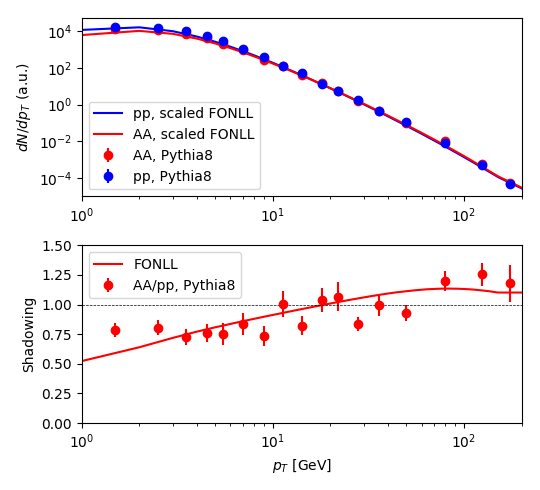
\includegraphics[width=.8\textwidth]{pythia-vs-fonll.png}
\caption[Top plot: a comparison of $D$-meson production in proton-proton]{Top plot: a comparison of $D$-meson production in proton-proton collisions (blue) and in Pb-Pb collisions (red) with cold nuclear matter effect only. FONLL calculations are shown as lines, and Pythia8 simulations are shown as symbols. Bottom plot: the ratio between the production in Pb-Pb collision (cold nuclear matter effect only) to the proton-proton baseline shows the nuclear shadowing effect.}
\label{fig:pythia-fonll}
\end{figure}

\section{Matching vacuum and medium-induced showers}
\subsection{Vacuum versus medium-induced shower phase-space}
\label{section:match}
The fate of vacuum-like showers in the hot-medium is complicated, and there have been studies for its phenomenological consequences \cite{Cao:2017zih,PhysRevLett.120.232001,PhysRevLett.120.232001,Caucal:2018ofz}.
The prescription that we build in this section is by no means exact, but follow the reasoning from a recent work \cite{PhysRevLett.120.232001}.
The general idea is to identify different regions of phase-space of radiation and apply different means of computation (DGLAP / transport) to different regions based on how much medium-modification it would have received.

\begin{figure}
\singlespacing
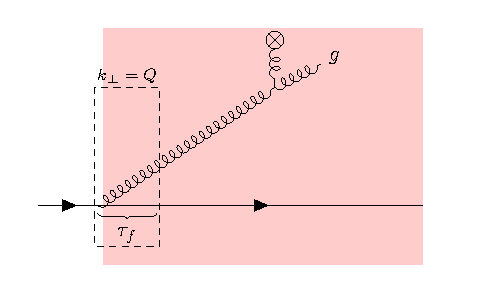
\includegraphics[width=.35\textwidth]{largeQ.pdf}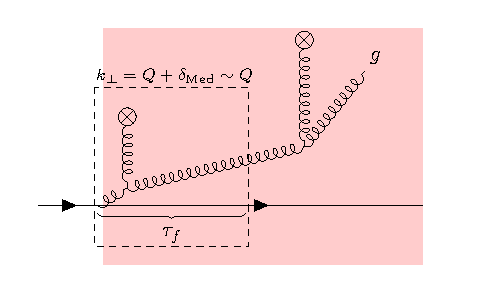
\includegraphics[width=.35\textwidth]{mediumQ.pdf}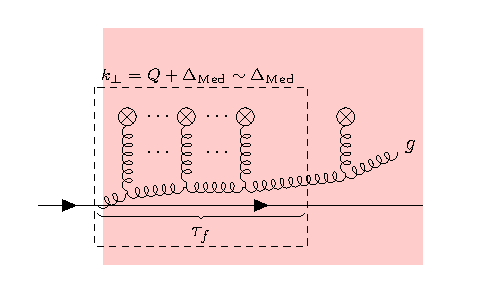
\includegraphics[width=.35\textwidth]{smallQ.pdf}
\caption[Demonstration of the medium corrections to vacuum-like radiation]{Demonstration of the medium corrections to vacuum-like radiation with different formation time. The energy of the gluon is held fixed, while the virtuality is decreasing from left to right.}
\label{fig:vac-med-interface}
\end{figure}

Consider a vacuum splitting of a hard parton that enters the medium at $z=0$.
The vacuum splitting has a formation time of $\tau_f \sim 2x(1-x)E/k_\perp^2$.
Before it fragments in the vacuum, the system (quark plus gluon) likely interacts with one or more scattering centers (labeled by ``i'') in the medium at time $t_i$.
Whether these interactions contribute coherently to the ``vacuum-like'' splitting follows the same argument as before.
Scatterings that are well-separated from the formation processes $\tau_f \ll t_i$ are treated as independent; they only broaden the transverse momentum without changing the radiation probability.
For $t_i \lesssim \tau_f$, the branching probability of the vacuum-like radiation gets modified.
Now classify the radiations using the average ``number'' of scatterings  $N = \tau_f/\lambda$ (for the case of a static medium).
\begin{itemize}
\item For a branching with large virtuality (left of figure \ref{fig:vac-med-interface}) so that $N \ll 1$ or equivalently $Q^2 \gg  g^2 x(1-x)E T$. 
The chance for a medium modification of the vacuum branching probability is negligible. 
\item Hold the energy of the radiation and decrease its virtuality (middle of figure \ref{fig:vac-med-interface}) so that $N = \tau_f/\lambda \sim 1$ ($Q^2 \sim g^2 x(1-x)E T$). 
Now, there is an order one probability of scatterings within $\tau_f$, but the initial virtuality still dominates the transverse momentum of the gluon.
The probability for the branching should also be modified accordingly, for example, using the higher-twist formula that expands in terms of $1/Q^2$.
\item Further decrease the initial virtuality of the branching (right of figure \ref{fig:vac-med-interface}) until $N \gg 1$.
Eventually, the medium broadening of the transverse momentum is large compared to the parton's virtuality from initial production.
It is proper to associate this parton an in-medium virtuality $Q^2 \sim g^2\sqrt{x(1-x)E T^3}$. 
When this happens, the branching probability gets heavily modified by the medium and should be replaced by a medium-induced radiation calculation.
\end{itemize}
Summarizing the two extreme regions:
The unmodified DGLAP evolution applies to the high-virtuality part of the shower ($Q^2 \gg \alpha_s \omega T$), while medium-induced calculation, via a transport equation, applies to the low-virtuality shower $Q^2 \sim \sqrt{\hat{q}\omega}$ (relation obtained in a static medium).
It is therefore natural to use the comparative relation between the partons' initial virtuality $Q^2$ and the transverse momentum change contributed by medium broadening $\Delta k_\perp^2 = (\mathbf{k}_\perp(\tau=\tau_f) - \mathbf{k}_\perp(\tau=0))^2$ to separate the medium-induced radiation from the vacuum-like radiation.
The matching prescription is then to cut-out the vacuum branchings generated by Pythia in the region $\Delta k_\perp^2 \gtrsim Q^2$, the cut region is referred to as the ``vetoed'' region in the literature \cite{PhysRevLett.120.232001}).
For a dynamical and fluctuating medium, there is no simple relation as $\Delta k_\perp^2\sim \sqrt{\hat{q}\omega}$ in the static medium, but the ``preformed parton'' technique can be used to determine $\Delta k_\perp^2$ self-consistently for each vacuum branching (to be explained in the next paragraph).
In a finite medium, certain vacuum-like branchings may have a long formation time that they form outside of the medium.
Due to the uncertainty principle, these branchings do not resolve the details of the medium, and their branching probability remains unchanged in our model.
This separate treatment of different regions of phase-space still depends on the detailed choice of the separation scale, so in the future, it would be desirable to develop a unified theoretical treatment for both vacuum and medium-induced showers in the time evolution picture.

Focusing only on the vacuum-like radiation generated by heavy quarks, one traces back a heavy quark line in the Pythia event recorder to find all the gluons from its final state radiation (FSR) and the original four-momentum of the heavy quark at the initial production vertex.
These FSR gluons are first treated as ``unformed'' by the transport models, and they are allowed to undergo elastic broadening with the medium.
In this way, by the time these gluons reaches their formation times ($t-t_0>\tau_f$), one knows both the initial virtuality of the splitting $Q^2$, as well as how much medium broadening $\Delta k_\perp^2$ it has acquired.
Then, applying our previous approximation, vacuum-like branching with 
$\Delta k_\perp^2 < R_v Q^2$ remains unmodified, but $\Delta k_\perp^2 > R_v Q^2$ vacuum branchings are rejected because these contributions are already taken care by the medium-induced rate in the transport model.
The order one $R_v$ parameter is introduced to parametrize the uncertainty in this matching scale.

\subsection{Visualizing the matching on the Lund diagram}
The Lund diagram is a useful tool to visualize the phase-space for high energy parton splitting.
There are many different choice of kinematic variables, but here we choose the vertical axis to be $Y = \ln(1/x) = \ln(E/\omega)$, and the horizontal 
axis to be $X = \ln(1/\theta^2) = \ln(\omega^2/k_\perp^2)$.
Here $x$ is the energy fraction carried by the daughter parton in a particular splitting, and $\theta$ is the daughter's emission angle relative to the mother parton.
This arrangement is inspired by the soft and collinear limit of the QCD splitting function (for example $q\rightarrow q+g$),
\begin{eqnarray}
dP^{q}_{qg} \sim \frac{\alpha_s C_F}{\pi} \frac{dx}{x}\frac{d\theta^2}{\theta^2} = \frac{\alpha_s C_F}{\pi} d\ln\frac{1}{x} d\ln\frac{1}{\theta^2}.
\end{eqnarray}
Therefore, the probability distribution of a vacuum-like splitting vertex should be uniform, apart from the running coupling effect.
The closer a point lies towards the origin, the higher its virtuality.
The soft and collinear radiations reside at large $X$ and $Y$.
Also, constant-formation-time contours are simply straight lines $Y+X=\ln(E\tau_f/2)$.

On the left of figure \ref{fig:lund}, we show the phase space occupied by the vacuum branching without a medium (left); on the right, it is medium-modified vacuum splitting (blue color map) and the medium induced radiation (red contour) from our simulation.
The simulation first identifies charm quarks with transverse momentum $90 < p_T <110$ GeV at the production vertex in Pythia, and then propagate them and their vacuum radiated gluons in a static medium with $T=0.3$ GeV with $\alpha_s = 0.3$ for a path length $L$.
We see that without the medium effect, the vacuum radiations fills the region bounded by the time-evolution limit $\tau_f < L$ (dash-dotted line) and the default non-perturbative bounds $k_\perp > 0.4$ GeV (dotted line) of Pythia. 
Inside the medium, the medium-induced radiations are distributed around the line $\tau_f\hat{q} = k_\perp^2$ which is $\theta^4\omega^3 = 2\hat{q}$ (dashed line) in the soft limit.  
However, this line is only an averaged estimation of the relation between $k_\perp, \omega$, and $\hat{q}$, since the actual outcome of the simulation strongly fluctuates.
The triangle area bounded by the line $\tau_f < L$ and the line $\theta^4\omega^3 = 2\hat{q}$ is where the vacuum-like radiation receives significant modification from medium interactions.
The rejection program introduced before suppresses the vacuum-like radiation in this region compared to the case without a medium.
Again, due to fluctuations, the triangular region is not entirely vetoed as the one demonstrated in \cite{PhysRevLett.120.232001}.

\begin{figure}
\singlespacing
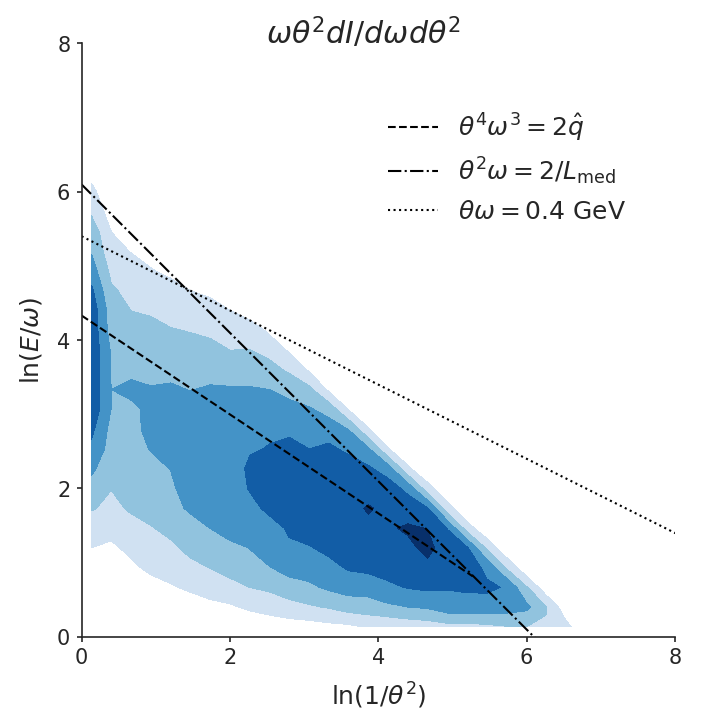
\includegraphics[width=.5\textwidth]{lund-vac.png}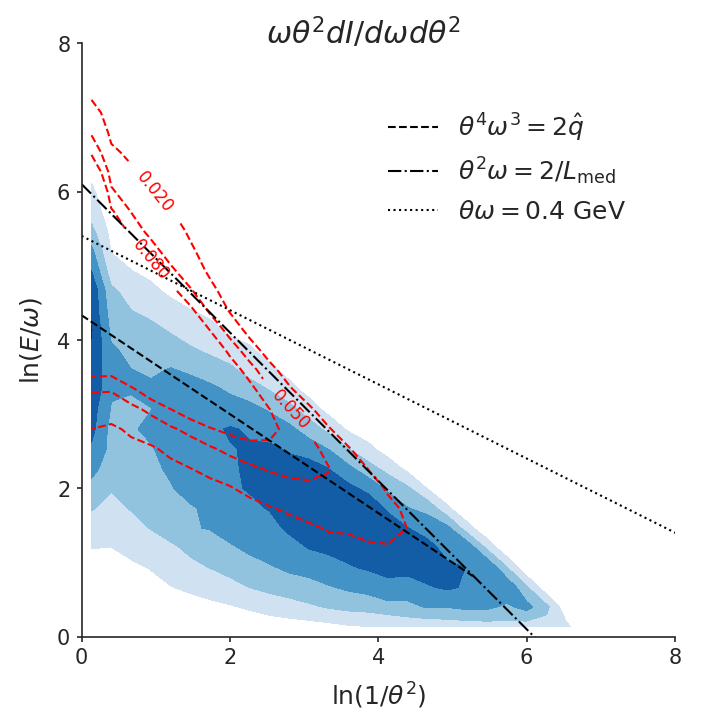
\includegraphics[width=.5\textwidth]{lund-med.png}
\caption[Plotting the gluon radiations from a charm quark on the Lund]{Visualize the gluon radiations from a charm quark on the Lund diagram. The gluon emission has an energy $\omega$ with angle $\theta$ with respect to the heavy quark. The blue heat map in the left plot shows the distribution of vacuum-like emissions without medium effects. The heat map in the right plot shows the distribution of vacuum-like emissions with medium effects; while the red contour stands for the medium induced emissions. Emissions on the black dashed lines have $k_\perp^2 = \sqrt{2\omega \hat{q}}$. Emissions on the dashed-dotted lines have a formation time equals to the medium path-length. Finally, the dotted line is the non-perturbative cut-off in Pythia $k_\perp = 0.4$ GeV.}
\label{fig:lund}
\end{figure}

Concluding this section, the realm of the transport equation and the DGLAP evolution is separated when the parton virtuality is comparable to the acquired transverse momentum broadening within the formation time.
High virtuality evolution is approximated as unmodified, while low virtuality evolution is terminated and replaced by the medium-induced processes via the transport evolution. 
This procedure is, of course, only viable if we initialize the simulation with a parton shower event generator.
We are not able to do such a separation using heavy quark spectra obtained from FONLL.

\section{Particles coupled to an evolving medium}
\label{section:couple-to-hydro}
The coupling between hydrodynamics and hard parton transport often requires switching of the reference frame, as the velocity of the medium local-rest-frame relative to the lab frame is a function of space-time.

\paragraph{For diffusion dynamics} The diffusion equations are most easily written in the local-rest-frame of the medium.
Given a particle's four momentum in the lab frame ($p_{L}^\mu$), one first boost it into the medium local-rest-frame ($p_{M}^\mu$),
\begin{eqnarray}
p_{M}^\mu &=& L^\mu_\nu(\vec{\beta}) p_{L}^\nu\\
L^\mu_\nu &=& 
\begin{bmatrix}
\gamma & -\gamma\vec{\beta}\\
-\gamma\vec{\beta} & \mathbb{1} + \frac{\gamma^2}{\gamma+1}\vec{\beta}\vec{\beta}
\end{bmatrix}
\end{eqnarray}
where $\vec{\beta}$ is the velocity of the fluid cell relative to the lab frame, and $L^\mu_\nu$ is the Lorentz transformation.
One needs to be careful with that since the time step in the fluid rest frame $\Delta t_{M}$ is different from the one in the lab frame $\Delta t_{L}$.
Consider the particle trajectory $\Delta x_{L}^\mu$ within $\Delta t_{L}$ observed in the lab frame and boost it into the medium frame,
\begin{eqnarray}
\Delta x_{L}^\mu = \frac{p_{L}^\mu}{E_L} \Delta t_{L} \xrightarrow{\textrm{boost}} \Delta x_{M}^\mu = \frac{L^\mu_\nu(\mathbf{v}_{M}) p_{L}^\nu}{E_L} \Delta t_L = \frac{p_{M}^\mu}{E_L} \Delta t_L
\end{eqnarray}
Comparing the time-component of the equations, one finds the time step in the medium frame being related to the lab frame step by the ratio between the energy of the particle in the two reference frames,
\begin{eqnarray}
\Delta t_M = \frac{E_M}{E_L} \Delta t_L
\end{eqnarray}
Once the momentum is updated in the medium frame to $p'_M$, it is boosted back to the lab frame,
\begin{eqnarray}
x'^{\mu} &=& x^{\mu} + \frac{p_{L}^\mu}{E_L} \Delta t_{L} \\
p_{L}^{'\mu} &=& L^\mu_\nu(-\vec{\beta}) p_{M}^{'\nu}
\end{eqnarray}
where we have chosen to update position before the update of the momentum.

The choice of $\Delta t_L$ is also tricky. 
Because the relativistic hydrodynamics for heavy-ion collision is usually solved in $(\tau,x,y,\eta_s)$ coordinates, the hydrodynamic fields are propagated from one constant proper time $\tau = \sqrt{t^2 - z^2}$ to the next.
As a result, there are two consequences if we use a straightforward uniform time step  $\Delta t_L$ for all particles:
\begin{itemize}
\item[1.] Different particles will be at different proper times $\tau$ at a constant $t$. It requires the program to load the entire hydrodynamic temperature and velocity history into the memory, which can be a memory storage problem for 3+1 D hydro simulation (the memory consumption for boost-invariant hydrodynamics is not critical).
\item[2.] The time step in the medium-rest-frame for particles at large space-time rapidity would be too small.
\end{itemize}
For these practical reasons, we choose to propagate particles with a constant proper-time step $\Delta \tau$. 
It requires the time step in the lab frame is different for each particle, depending on its location and momentum. The time-step is solved by,
\begin{eqnarray}
\Delta \tau = \sqrt{(t+\Delta t_L)^2 - (z+v_z \Delta t_L)^2} - \sqrt{t^2 - z^2}.
\end{eqnarray}
This is (keeping the positive solution),
\begin{eqnarray}
\Delta t_L(p, x) = \frac{-(t-z v_z) + \sqrt{(t-z v_z)^2 - (1-v_z^2)(\Delta \tau^2 + 2\sqrt{t^2 - z^2}\Delta \tau )}}{2(1-v_z^2)}
\label{eq:dt-transformation}
\end{eqnarray}
This adaptive time step propagates a particle between constant proper-time hyper-surfaces, therefore only two steps of hydrodynamic information needs to be loaded into memory at any given time.
Also $\Delta t_L$ becomes larger for forward/backward particles.

\paragraph{For matrix-element scattering} Sampling matrix-element-based scattering is more complicated than solving the diffusion equation.
One can straightforwardly sample the initial state in the medium local-rest-frame, but the final state is most efficiently sampled in the center-of-mass frame of the few-body collisions.
The center-of-mass velocity relative to the local-rest-frame is,
\begin{eqnarray}
\vec{\beta}_{C} = \frac{\sum_{i\in \textrm{IS}} \vec{p}_i}{\sum_{i\in \textrm{IS}} E_i}
\end{eqnarray}
where ``IS'' stands for the initial state.
\begin{itemize}
\item[1.] For each hard parton, determine $\Delta t_L$ with equation \ref{eq:dt-transformation}.
\item[2.] Boost the particle to the medium rest-frame and sample the scattering rate $\Delta t_M R$ channel, and then sample the initial-state medium parton(s).
\item[3.] In the CoM frame of the initial state, sample the final state particles.
\item[4.] Boost back the final state particles to the medium rest frame.
\item[5.] Boost back to the lab frame.
\end{itemize}

\section{Heavy-flavor hadronization and hadronic stage}
\label{section:hadronization}
At a temperature near $T_c$, light hadrons can be sampled from the hydrodynamics energy-momentum tensor statistically.
For hard partons that may be off equilibrium, a microscopic hadronization model is in need.
The final hadronic system is also dense enough for the heavy hadron to interact.
Though the hadronic interactions are not analyzed as extensively as the QGP interaction, studies have shown hadronic rescatterings contribute to finite low-$p_T$ $v_2$ of D-mesons \cite{Cao:2015hia}.
Therefore we also include the afterburner stage for the heavy flavors.

\subsection{The instantaneous approximation of hadronization} 
The hadronization implementation is described in \cite{Cao:2013ita}.
It combines the fragmentation of heavy quarks at high momentum and the recombination with medium partons into hadrons at low momentum.
The hadronization is treated to be instantaneous on an isothermal hypersurface.
This instantaneous approximation has certain drawbacks.
First, hadronization is a long-distance process. 
In the rest frame of the heavy flavor, it takes time on a scale of $1/\Lambda_{QCD}$. 
With a large boost factor $E/M_H\sim E/M_Q$, the formation time of the heavy hadron can be comparable to macroscopic length scales.
For example, for a moderate $E=10$ GeV charm quark with $M_Q=1.3$ GeV, this time is estimated to be $8$ fm/$c$, which is certainly not instantaneous, considering the hydrodynamic stage only last for $O(10)$ fm/$c$.
Second, an instantaneous recombination process breaks energy conservation and the detailed balance.
To solve all of these problems, one may need to consider using a dynamical hadronization model \cite{He:2019vgs}.

\paragraph{Fragmentation} 
In high energy electron-positron collisions and proton-proton collisions, high momentum heavy quarks hadronize through the fragmentation mechanism.
The energetic heavy quark produces a bunch of hadrons with a heavy hadron that carries a certain fraction of the origin quark momentum $z = p_H/p_Q$.
The probability distribution of $z$ is known as the fragmentation function $D(z)$, and can be measured in, e.g., electron-positron colliders.
There are different parametrizations for $D(z)$ and the Peterson fragmentation function \cite{PhysRevD.27.105} is used in the present study,
\begin{eqnarray}
D(z) \propto \frac{1}{z(1-\frac{1}{z} - \frac{\epsilon}{1-z})^2}
\end{eqnarray}
where $\epsilon$ is a parameter that scales as $m_Q^{-2}$ ($\epsilon_c \approx 0.05, \epsilon_b \approx 0.006$).

\paragraph{Recombination}
In proton-proton collisions, heavy quarks can hadronize into mesons by the recombination with a light quark in the proton remnant \cite{Mehen:2003rf}.
In a heavy-ion collision, the recombination mechanism plays a far more essential role for low $p_T$ heavy flavors, given the abundance of thermal medium partons.
Early studies in nuclear collisions \cite{Oh:2009zj} assumed that the recombination probability can be computed from the wave function overlap between initial state partons and final state mesons or baryons, with the momentum of the medium parton integrated over the thermal distribution.
\begin{eqnarray}
\frac{dP_M(p', p)}{dp'^3} &=& \int dk^3 n_{\bar{q}}(k) W_{M}(p, k)\delta^{(3)}(\vec{p}'-\vec{p}-\vec{k}), \label{eq:meson_recombine}\\
\frac{dP_B(p', p)}{dp'^3} &=& \int dk_1^3 dk_2^3 n_{\bar{q}}(k_1)  n_{\bar{q}}(k_2) W_{B}(p, k_1, k_2)\delta^{(3)}(\vec{p}'-\vec{p}-\vec{k}_1 - \vec{k}_2), \label{eq:baryon_recombine}.
\end{eqnarray}
On the left are the differential probability for a heavy quark with momentum $p$ to hadronize into a heavy meson (first line) or a heavy baryon (second line) with momentum $p'$ through recombination.
They are equal to integration of light quark(s)/antiquark(s) momenta of the produced baryon/meson Wigner function $W$ times the thermal distribution function, subjected to three-momentum conservation.
The energy conservation is not imposed in the instantaneous $2\rightarrow 1$ coalescence approach.
The quark/antiquark distribution function is the Fermi-Dirac one, neglecting the chemical potential, 
\begin{eqnarray}
n = \frac{g_q V}{e^{\beta p\cdot u} + 1}
\end{eqnarray}
with $u$ the fluid velocity and $p$ the four momentum of the light quark / anti-quark.
$g$ is the degeneracy factor of the quark, and $V$ is a test volume that will eventually be canceled by the normalization factor in the Wigner function.
As a remark, we have assumed in the transport model that medium partons are massless because the thermal masses are higher-order effects for energy loss; but for recombination into bound states near $T_c$, it is crucial to use non-perturbative constituent masses of light quarks $m_u = m_d = 300$ MeV and $m_s = 475$ MeV.

Regarding the meson wave-function, there have been efforts using the Dirac equation to obtain a more realistic wave-function for different states of heavy mesons \cite{Zhao:2018jlw,PhysRevD.88.014021}.
The current model uses a parametrized Gaussian wave-function for simplicity,
\begin{eqnarray}
\phi_M(\vec{r}) &=& \left(\frac{1}{\pi \sigma^2}\right)^{3/4} e^{-\frac{r^2}{2\sigma^2}}.
\end{eqnarray}
$\sigma$ is related to the reduced mass of the two body system $\mu = m_1 m_2/(m_1+m_2)$ and the frequency of the  two-body potential $\omega$ by $\sigma = 1/\sqrt{\mu \omega}$.
These frequencies are estimated from the charge radius of different heavy mesons: $0.106$ GeV for charmed mesons and $0.059$ GeV for the bottom mesons.
The Wigner function is defined in terms of the relative distance $\vec{r}$ and relative momentum $\vec{q}$ between the quark and anti-quark,
\begin{eqnarray}
W_M(\vec{r}, q^2) &=& g_M \int d^3 \vec{a} e^{-i\vec{q}\cdot \vec{a}} \phi_M(\vec{r}+\vec{a}/2) \phi_M^*(\vec{r}-\vec{a}/2) \\
\vec{q} &=& \frac{E_2\vec{p}_1 - E_1\vec{p}_2}{E_1+E_2}.
\end{eqnarray} 
Averaging over the light quark's positions,
\begin{eqnarray}
W_M(q^2) &=& \frac{g_M}{V} (2\sqrt{\pi}\sigma)^3 e^{-\sigma^2 q^2},
\end{eqnarray}
which is the quantity needed in equation \ref{eq:meson_recombine},
\begin{eqnarray}
\frac{dP_M(p',p)}{dp'^3} &=& \int dk^3 \frac{g_q g_M}{e^{\beta p\cdot u} + 1} (2\sqrt{\pi}\sigma)^3 e^{-\sigma^2 q^2} \delta^{(3)}(\vec{p}'-\vec{p}-\vec{k}),
\end{eqnarray}
where the test volume in the distribution function has been canceled by the one in the Wigner function.

The same procedure applies to heavy baryons, with the three-body Wigner function in the Gaussian approximation as,
\begin{eqnarray}
f_B^W(q_1^2, q_2^2) = \frac{N g_B}{V^2} (2\sqrt{\pi\sigma_{1,2}\sigma_{12,3}})^6 e^{-q_{1,2}^2 \sigma_{1,2}^2 - q_{12,3}^2 \sigma_{12,3}^2}.
\end{eqnarray}
The relative momenta are defined as,
\begin{eqnarray}
\vec{q}_{1,2} &=& \frac{E_2 \vec{p}_1 -E_1\vec{p}_2}{E_1+E_2},\\
\vec{q}_{12,3} &=& \frac{E_3 (\vec{p}_1+\vec{p}_1) - (E_1+E_2)\vec{p}_3}{E_1+E_2 + E_3},
\end{eqnarray}
and the $\sigma$ related to the frequency and masses by,
\begin{eqnarray}
\sigma_{1,2}^{-1} &=& \sqrt{\omega \frac{m_1m_2}{m_1+m_2}}\\
\sigma_{12,3}^{-1} &=& \sqrt{\omega \frac{(m_1+m_2)m_3}{m_1+m_2+m_3}}
\end{eqnarray}

To synthesize these two competing mechanisms of hadronization, first, one samples the recombination probability in equations \ref{eq:meson_recombine} and \ref{eq:baryon_recombine} and determines whether the heavy quark coalesces with medium partons. 
If not, its hadronization will be handled by the Pythia fragmentation routine with the Peterson fragmentation function.

\subsection{Hadronic rescattering of heavy-meson in UrQMD}
Currently, UrQMD includes hadronic collisions between charmed mesons and $\pi$, $\rho$ mesons.
These cross-sections are obtained in \cite{Lin:2000jp}.
Hadronic cross-section of the charmed baryons and bottom hadrons are not included.

One modification made to the UrQMD heavy-flavor sector is that the kinematic effect of backreaction from heavy flavor mesons on the light sector is turned-off. 
It is achieved by resetting the light scattering partner's four-momentum back to its initial value.
This practice retains the same level of approximation of the linearized transport equation in the QGP phase and allows for an easy oversampling of the number of heavy flavor particles to obtain better statistics.

\section{Benchmark calculation of observables}
\label{section:benchmark}
In the last section of this chapter, we provide a benchmark calculation of the open-heavy flavor simulation framework by comparing to experimental data. 
A systematic calibration of model parameters and uncertainties will be discussed in the next two chapters.

\subsection{Open heavy flavor observables}
Experimentally, the ground states mesons $D^0, \bar{D}^0, D^{\pm}, B^{\pm}, D_s^{\pm}, B_s^{\pm}$ and the excited states $D^{*\pm}$ can be measured. 
Their nuclear modification factor and momentum anisotropy have been measured at both LHC and RHIC.
Currently, we focus on comparing to non-strange $D$ and $B$ mesons data.
Though strange heavy mesons $D_s, B_s$ are also very interested as they contain the strangeness enhancement information, the strangeness physics is not the main focus of this work.

The nuclear modification factor has already been introduced in chapter \ref{chapter:introduction}. 
Here we summarize how the momentum anisotropy observables are computed.
A list of the measurements and references can be find in table \ref{table:ALICE-obs} and table \ref{table:CMS-obs}.
\begin{center}
\begin{table}[h]
\caption{ALICE dataset}\label{table:ALICE-obs} 
\begin{tabularx}{\columnwidth}{XXX}
\hline 
 Observables & Centrality & Reference\\ 
\hline 
$D$-meson $v_2$ & 30-50\% & \cite{Acharya:2017qps}\\ 
\hline 
Event-engineered $D$-meson $v_2$ & 30-50\% & \cite{Grosa:2017zcz}\\ 
\hline 
$D$-meson $R_{AA}$ & 0-10, 30-50, 50-80\% & \cite{Acharya:2018hre}\\
\hline 
\end{tabularx}
\end{table}
\begin{table}[h]
\caption{CMS dataset}\label{table:CMS-obs} 
\begin{tabularx}{\columnwidth}{XXX}
\hline 
Observables & Centrality & Reference\\ 
\hline 
D${}^0$-meson $v_2$ & 0-10, 10-30, 30-50\% & \cite{Sirunyan:2017plt}\\ 
\hline 
D${}^0$-meson $R_{AA}$ & 0-10\%, 0-100\% & \cite{Sirunyan:2017xss}\\ 
\hline 
B${}^{\pm}$-meson $R_{AA}$ & 0-100\% & \cite{Sirunyan:2017oug}\\ 
\hline 
\end{tabularx}
\end{table}
\end{center}

\paragraph{Momentum anisotropy}
Heavy flavor momentum anisotropy at high-$p_T$ is thought to be the result of anisotropic energy loss because on average, hard partons emitted along the short axis lose less energy than those emitted along the long axis.
At low momentum, the momentum anisotropy is related to collective flow since the heavy quark interacts so frequently with the medium and tends to catch up with the flow velocity of the medium.
Both mechanisms produce $v_2$ relative to the common reference frame of the bulk geometry/bulk flow.
The $p_T$ differential $v_2$ is usually measured in a two-particle correlation approach,
\begin{eqnarray}
v_n\{2\}(p_T) = \frac{\mathfrak{Re}\langle d_n\{2\} \rangle}{\langle c_n\{2\}\rangle}.
\end{eqnarray}
$c_n$ is the event-wise two particle correlation of $N$ reference particles (REF, the bulk medium) within a certain kinematic range,
\begin{eqnarray}
c_n &=& \frac{|Q_n|^2 - N}{N(N-1)},  \\
Q_n &=& \sum_{i=1}^N e^{i n \phi},
\end{eqnarray}
and the event average ($\langle\cdots\rangle$) is weighted by $N(N-1)$.
$d_n$ is the correlation between the $M$ particles of interest (POI, in this case the heavy flavors) and the $N$ reference particles,
\begin{eqnarray}
d_n &=& \frac{q_n Q_n^* - m}{MN-m},  \\
q_n &=& \sum_{j=1}^M e^{i n \phi}
\end{eqnarray}
$m$ is the number of POI that is also counted as REF to subtract auto-correlations. 
The event average is weighted by the number of pairs $MN-m$.

\paragraph{Event-shape engineering on heavy-flavor $v_2$}
Event-shape engineering is a more recent idea to look at the detailed response of the hard sector to the medium geometry.
Experimentally, an ensemble of events belonging a certain centrality class is further classified according to its ``event shape'', measured by $q_2$,
\begin{eqnarray}
q_2 = \frac{|Q_2|}{\sqrt{N}}.
\end{eqnarray}
Due to event-by-event geometry fluctuations, the event shape in a given centrality class can vary dramatically.
The ALICE experiment then measures the D meson $v_2$ with events having the $20\%$ largest $q_2$ and events with the $60\%$ smallest $q_2$.
They found a large separation between the resulting $v_2$ of bias selected events compared to the $v_2$ calculated from unbiased events.
This measurement quantifies the response of the hard probe to the event geometry fluctuation while controlling multiplicity. 

\subsection{A first comparison to data}
We do not intend to optimize all the parameters in the model in this first comparison to data, but use a reasonable estimate of the parameters to understand the model.
The \trento\ parameters and the hydrodynamic transport coefficients are obtained from the high likelihood parameters in \cite{Bernhard:2018hnz}.
The heavy quarks start to lose energy from $0.6$ fm/$c$, and the matching condition between the vacuum-like radiation and the medium-induced radiation is $\Delta k_\perp^2 = R_v Q^2$ with $R_v = 1$.
We used only leading order contributions from the weakly coupled theory, and try both fixed coupling and running coupling.
The default switching scale between a large-$Q$ scattering small-$Q$ is $Q_{\textrm{cut}}^2 = 4 m_D^2$.

\begin{figure}
\singlespacing
\centering
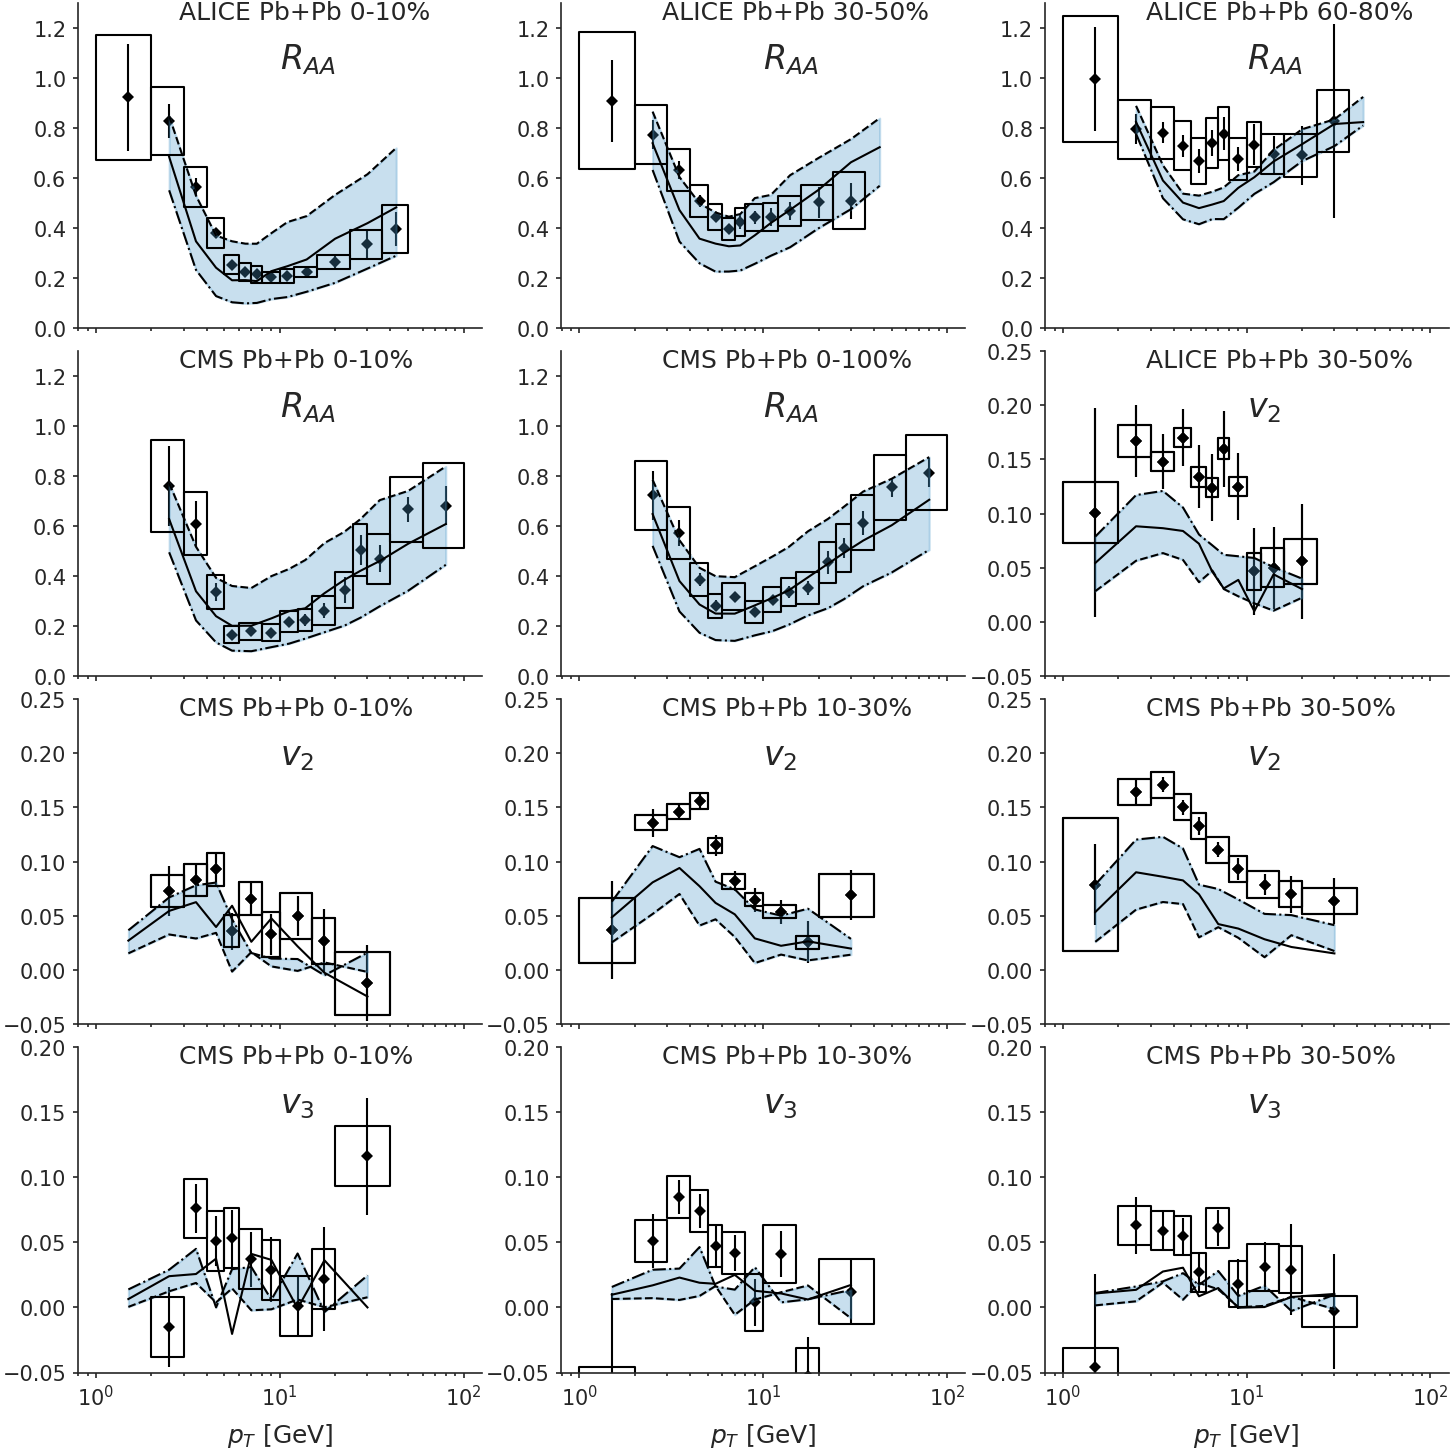
\includegraphics[width=\textwidth]{fix_alphas.png}
\caption[Benchmark results using a fixed coupling constant $\alpha_s = 0.2$ (dashed),]{Benchmark results using a fixed coupling constant $\alpha_s = 0.2$ (dashed), $0.3$ (solid), and $0.4$ (dash-dotted). The blue bands fill between the results using $\alpha_s=0.2$ and $0.4$. They are compared to the experimental data (black symbols) obtained by the ALICE Collaboration \cite{Acharya:2017qps,Acharya:2018hre} and the CMS Collaboration \cite{Sirunyan:2017xss,Sirunyan:2017plt}.}
\label{fig:new:fix-a}
\end{figure}

\paragraph{Fixed coupling} First, we compute with a fixed coupling constant.
It is understood as an effective in-medium coupling for both elastic and radiative processes.
In figure \ref{fig:new:fix-a}, we present the results (lines and bands) with data points measured at $\sqrts{s} = 5.02$ TeV for D mesons (symbol with error bars and boxes).
Different line shapes corresponds to different coupling $\alpha=0.2$ (dashed), $0.3$ (solid), and $0.4$ (dash-dotted). 
The types of observables are shown within each subplot, indicating the experimental collaboration, the collision system, and the centrality.

Looking at the experimental measurements, $R_{AA}$ increases with the centrality classes and displays a minimum around $8 < p_T < 10$ GeV.
At high-$p_T$, the $R_{AA}$ increases slowly towards the baseline around one, noticing the log-scale of $p_T$.
At low-$p_T$, the $R_{AA}$ quickly rises.
There are many reasons for this, for example, the feed down from higher-$p_T$ particles due to energy loss;  the feeding from low-$p_T$ particles that are pushed outward by the strong medium radial flow.
Besides, the recombination hadronization mechanism also plays a part, as the D meson is gaining momentum (on average) in the recombination process.
Based on the comparison to $R_{AA}$, a phenomenological value for a fixed $\alpha_s$ is around $0.3$--$0.4$.
However, such values cannot explain the large momentum anisotropy in mid-central collisions, e.g., centrality 30-50\%.
This is usually referred as the $D$ meson $R_{AA}$--$v_2$ puzzle, which also appears for leading light hadrons.
There have been different solutions proposed to this problem, such as a sudden increase in the interaction strength near $T_c$, fine-tuning the general temperature-momentum dependence of the transport coefficients, et cetera. \cite{SCARDINA2016329,Xu:2017obm,Shi:2018vys}.
In the next two chapters, we will see if this discrepancy can be overcome by a fine-tuning of parameters in the current model.
A non-zero $v_3$ of $D$ mesons is evidence of heavy-flavor coupling to detailed event-by-event nuclear geometry fluctuations.
The calculation of $v_3$ is systematically below the data, despite the considerable statistical and systematic uncertainty.

\begin{figure}
\singlespacing
\centering
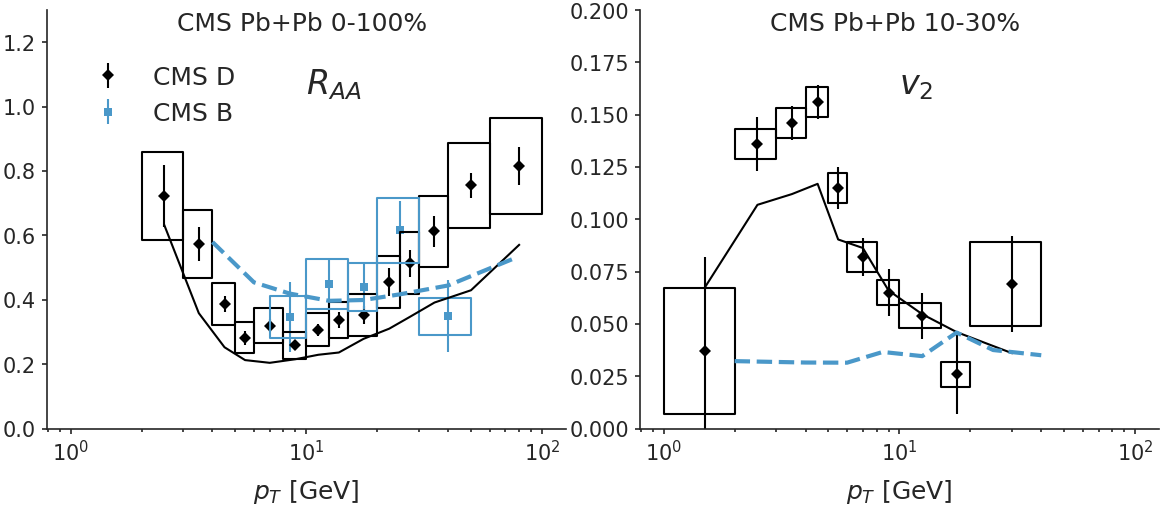
\includegraphics[width=\textwidth]{run_alphas_DB.png}
\caption[Demonstrating the mass dependence of the observables using]{Demonstrating the mass dependence of the observables using $\alpha_s = 0.4$. 
The D meson and B meson results are labeled by black and blue, respectively.
Left plot: $R_{AA}$ for 0-100\% centrality. Right plot: $v_2$ for 10-30\% centrality.}
\label{fig:new:charm-bottom}
\end{figure}

In figure \ref{fig:new:charm-bottom}, we compare the calculation with $\alpha_s = 0.4$ for charmed meson $R_{AA}^D$ and bottom meson $R_{AA}^B$ at $0-100\%$ centrality and D meson and B meson flow at $10-30\%$ centrality.
The mass effect of bottom quarks is much stronger than for charm quarks; therefore, $R_{AA}^B$ at intermediate $p_T$ is higher than $R_{AA}^D$. 
At very high $p_T$, the ``dead cone'' of bottom quark becomes insignificant, and the $B$ and $D$ meson $R_{AA}$ converge.
Unlike the sudden increase of $v_2^D$ at low $p_T$, $v_2^B$ is always small, meaning that the bottom quarks do not catch up to the medium flow as the charm quarks do and remain far from equilibrium.

\begin{figure}
\singlespacing
\centering
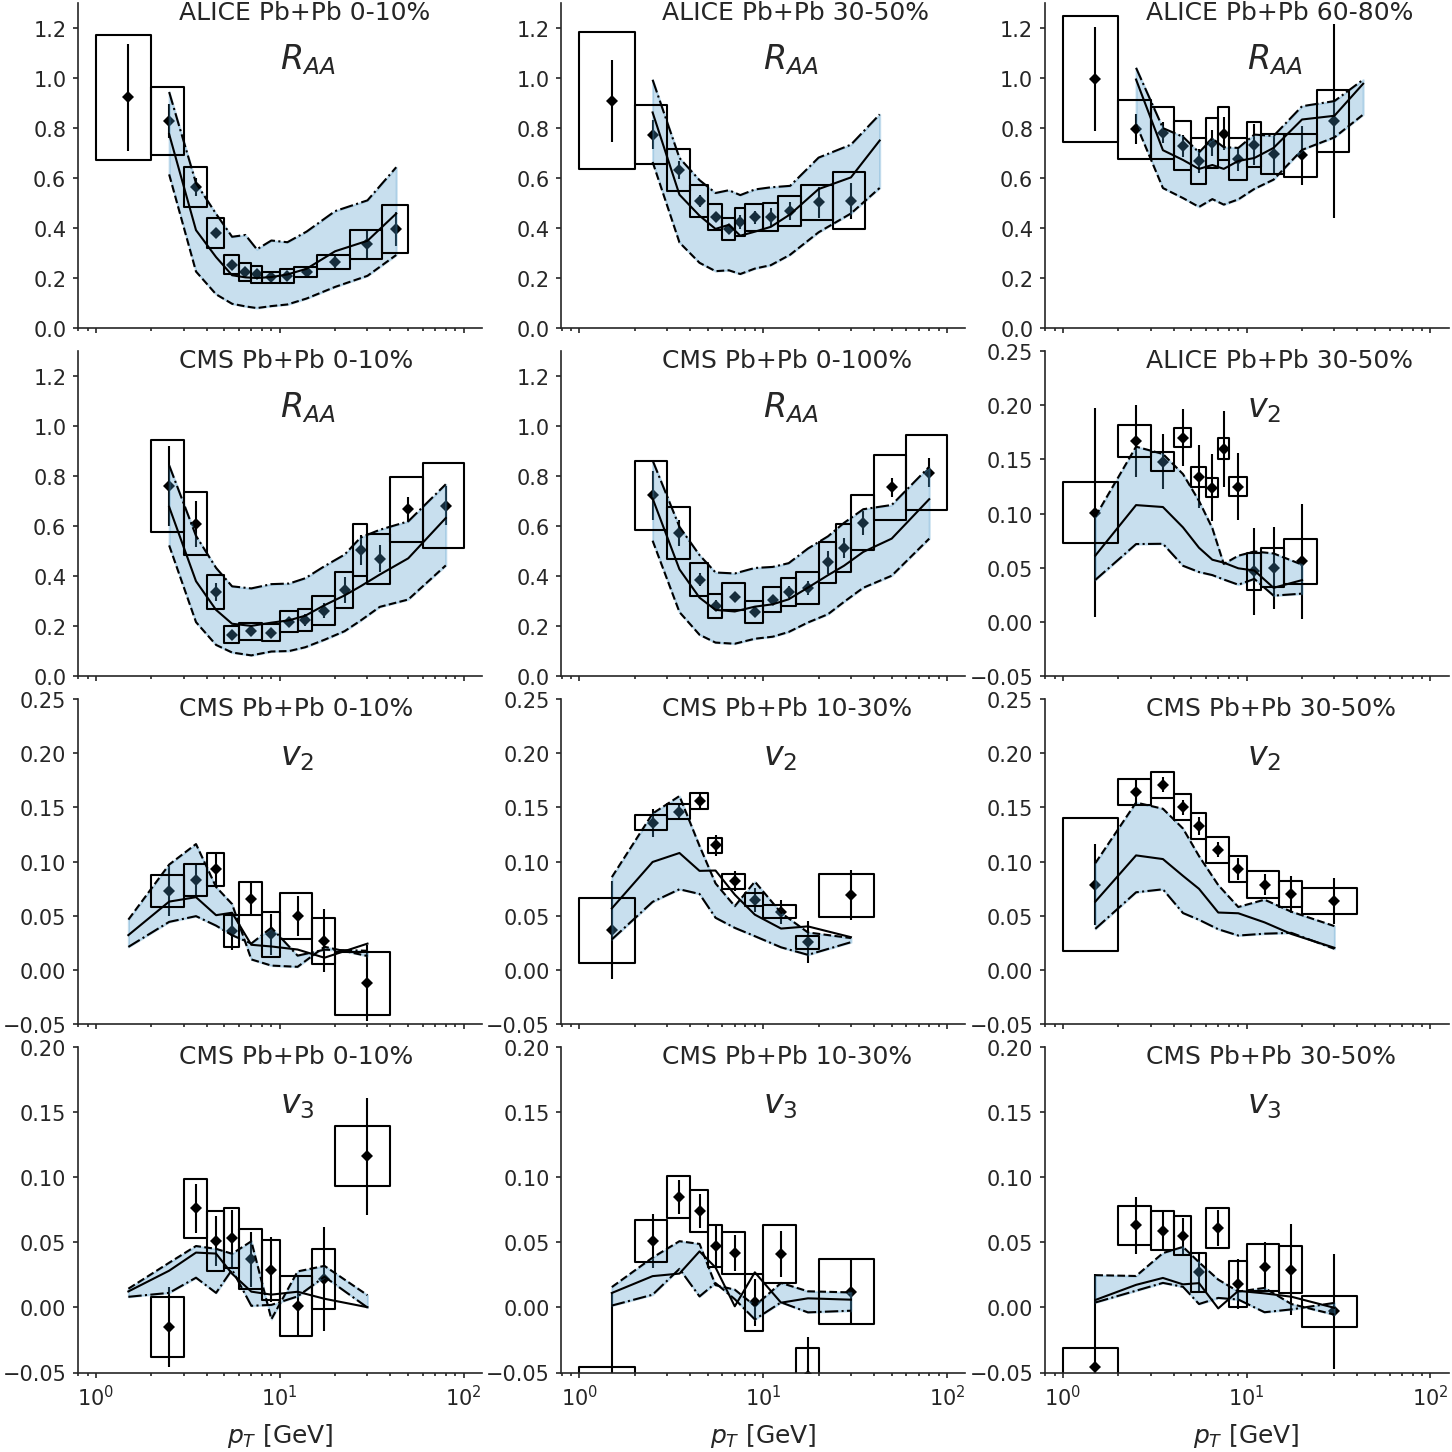
\includegraphics[width=\textwidth]{run_alphas.png}
\caption[Benchmark results using a running coupling constant. The]{Benchmark results using a running coupling constant. The medium scale that stops the low-$Q$ running is chosen at $Q_{\textrm{med}} = \mu\pi T = \pi T$ (dashed), $2\pi T$ (solid), and $4\pi T$ (dash-dotted). They are compared to the experimental data (black symbols) obtained by the ALICE Collaboration and the CMS Collaboration.}
\label{fig:new:run-a}
\end{figure}

\paragraph{Running coupling} Moving to a running coupling constant, the uncertainty of the in-medium coupling strength is transferred to the uncertainty of the medium scale in the running $\alpha_s$,
\begin{eqnarray}
\alpha_s(Q) = \frac{2\pi}{9}\frac{1}{\ln \left( \max\{Q, \mu\pi T\} / \Lambda\right)}.
\end{eqnarray}
Due to the running, heavy quark radiation at high energy will be reduced compared to low energy and the interaction strength with the medium is enhanced at low temperature relative to high temperature.

In the comparison shown in figure \ref{fig:new:run-a}, we choose $\mu = 1, 2, 4$, terminating the low-$Q$ running of $\alpha_s$ at $Q = \pi T$ (dashed), $2\pi T$ (solid), $4\pi T$ (dash-dotted).
We use $\pi T$ as a natural unit because it is the typical thermal scale in the finite-temperature field theory calculations.
Given that the entire heavy-flavor coupled-to hydrodynamic model is only an approximation, one should not think of the appearance of $\pi$ so seriously.
The $\mu=2\pi T$ choice explains the nuclear modification factor for all centralities very well but underestimates $v_2$ by 50\%.
The $\mu=\pi T$ case achieves a better agreement with $v_n$, but $R_{AA}$ is systematically off.
Therefore, going from fixed coupling to running coupling, the $v_2$ puzzle remains.

\begin{figure}
\singlespacing
\centering
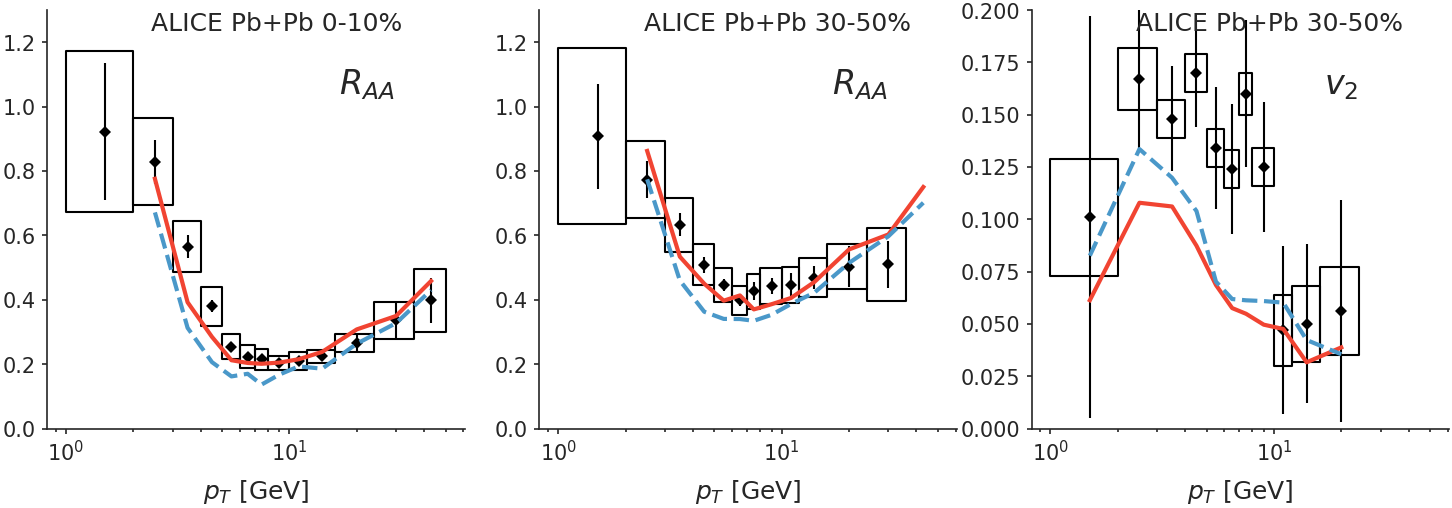
\includegraphics[width=\textwidth]{run_alphas_cut.png}
\caption[Effect of changing the switch scale between small-$Q$ diffusion]{Effect of changing the switch scale between small-$Q$ diffusion modeling and large-$Q$ scattering modeling. $\mu=2$ is used. The red solid lines used a switching scale at $Q_{\textrm{switch}}^2 = 4 m_D^2$, and the blue dashed lines uses $16 m_D^2$.}
\label{fig:new:run-cut}
\end{figure}
\paragraph{Switching scale dependence} By construction, the energy loss should be insensitive to the switching scale between the small-$Q$ diffusion and the large-$Q$ scattering in the high energy, weakly coupled limit.
We check if this arguments holds for phenomenological application.
In figure \ref{fig:new:run-cut}, in addition to the default $Q_\textrm{cut}^2 = 4 m_D^2$ (red solid lines), we also use $Q_\textrm{cut}^2 = 16 m_D^2$ (blue dashed lines) to model an increase amount of probe-medium interaction by diffusion compared to scattering.
We find that the effect on high-$p_T$ observable is small.
Because the high-$p_T$ dynamics is dominated by the radiative energy loss, whose $Q_\textrm{cut}$ is indeed small as checked in chapter \ref{chapter:transport}.
Larger differences of $R_{AA}$ and $v_2$ is observed at low-$p_T$.
One reason for this is that the $Q_\textrm{cut}$ independence argument obtained for high energy partons does not work very well for low-velocity partons.
Another reason is that despite the scattering dynamics and the diffusion dynamics having a matched diffusion constant (second moment of the momentum transfer), they are differed in all other higher moments, in particular, the drag (first moment).
Remember that the drag coefficient in the diffusion dynamics is not a direct input from the weakly coupled theory, but is determined by the Einstein relation.
The Einstein relation only guarantees that the diffusion dynamics evolve the system to the same equilibrium as the scattering dynamics, but the non-equilibrium path it takes can be very different from that of the scattering dynamics.

This $Q_\textrm{cut}$ dependence may be undesirable at first sight, but one knows that the weakly coupled scattering picture does not necessarily work for the phenomenological coupling regime ($g\sim 2$), while the diffusion dynamics can be extended to the strongly coupled regime.
The $Q_\textrm{cut}$ parametrizes an important source of theoretical uncertainty in our modeling.

\begin{figure}
\singlespacing
\centering
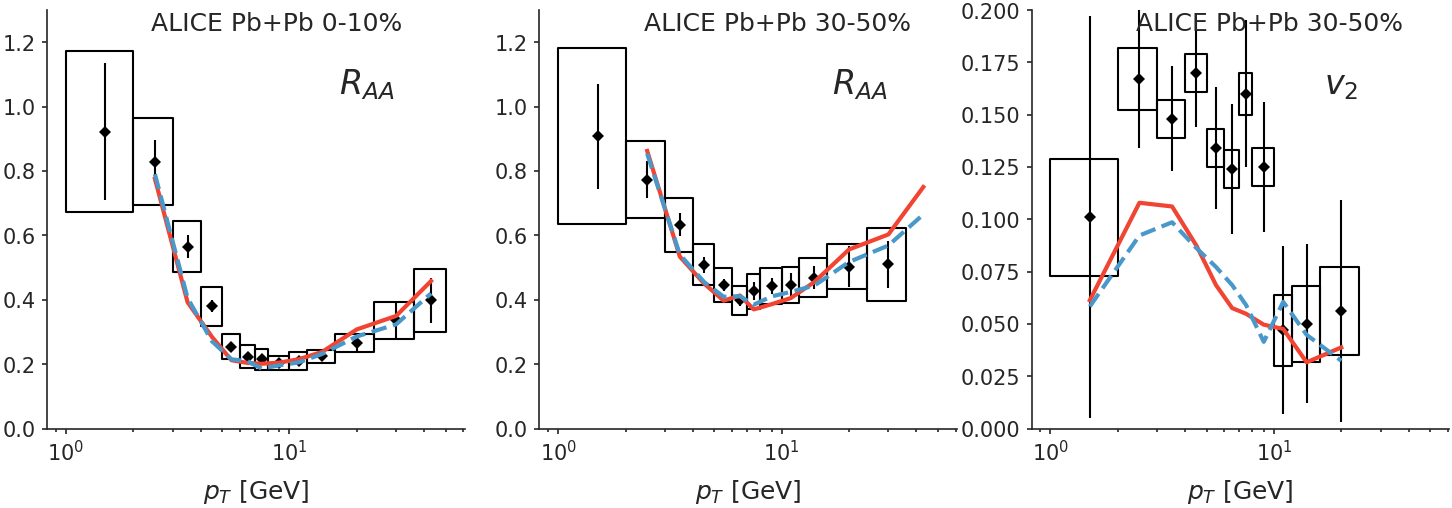
\includegraphics[width=\textwidth]{run_alphas_match.png}
\caption[Effect of changing the matching scale parameter $R_v$]{Effect of changing the matching scale parameter $R_v$ ($\Delta k_\perp^2 = R_v Q^2$) between the vacuum-like shower and the medium-induced shower. $\mu=2$ is used. The red solid lines use $R_v =1$, while the blue dashed lines use $R_v = 1000$, which leave the vacuum-like shower largely unmodified.}
\label{fig:new:run-match}
\end{figure}

\paragraph{Vacuum / medium-induced radiation matching scale dependence}
As explained, there are separated treatments of radiation in different regions of phase-space on the Lund-diagram.
Accordingly, we need to subtract the vacuum radiation that overlaps with the medium-induced region in the Pythia event generator.
In our earlier transport study of heavy flavor \cite{Ke:2018tsh}, this subtraction was not included; therefore, we would like to demonstrate the impact of this mistreatment here.

In figure \ref{fig:new:run-match}, two calculations are shown. 
The red dashed lines stand for the case where we removed vacuum-like radiations that satisfy $\Delta k_\perp^2 > Q^2$.
The solid blue lines are calculations without this subtraction.
The two calculations for $R_{AA}$ only differ for $p_T\gtrsim 20$ GeV, because only high-$p_T$ heavy quarks can undergo splittings that take long enough time to receive significant medium corrections.
Also, the difference is larger for central collisions than for peripheral collisions, because medium the effect for the latter is weaker.
No significant difference is observed for $v_n$.

\begin{figure}
\singlespacing
\centering
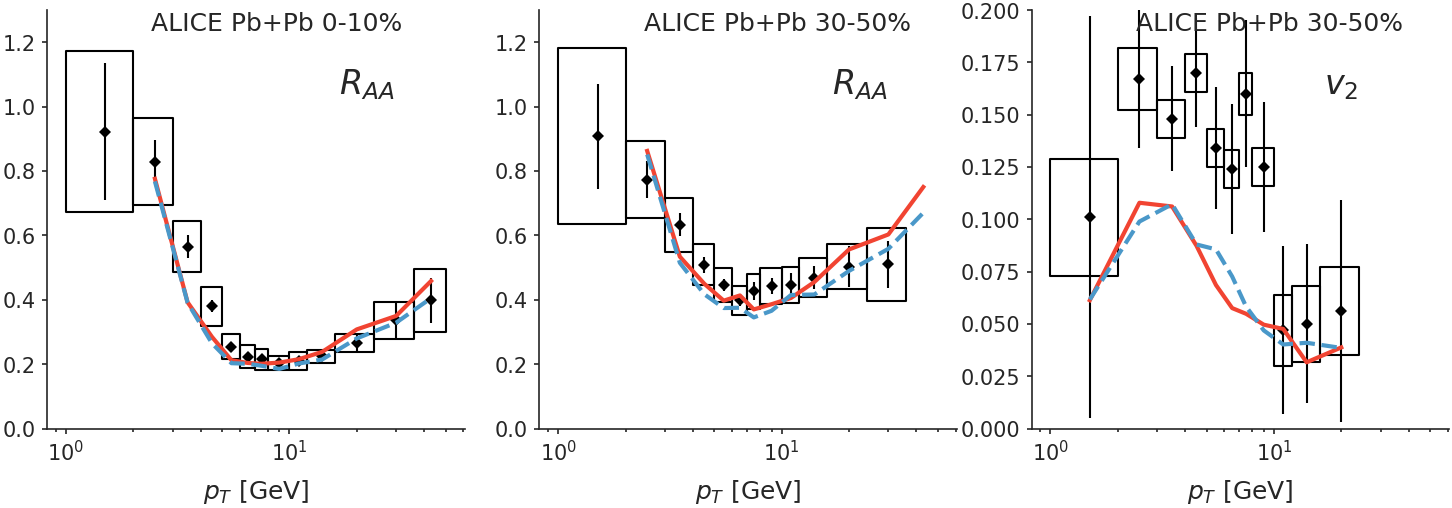
\includegraphics[width=\textwidth]{run_alphas_local.png}
\caption[The impact of using the ``local rate'' approximation. The red]{The impact of using the ``local rate'' approximation. The red solid lines use the default implementation; while the blue dashed lines perform the rescatterings in an imaginary infinite box using locally defined temperatures to mimic the ``local rate'' approximation.}
\label{fig:new:run-local}
\end{figure}

\paragraph{Performance of the ``local rate'' approximation}
Finally, it is interesting to examine the effect of an ``local rate'' approximation of the radiative processes on the observables.
It approximates the radiation probability in a medium with slowly varying temperature by the integration of radiation rates defined in an infinite static box with the local temperature at each point.
One can also refer to it as the ``adiabatic'' approximation because it assumes the temperature variation is slow compared to the formation time.

We know this approximation can be broken by the fast expansion of the QGP fireball and would like to quantify the impact.
It is easy to mimic the ``local'' approximation in our model; one can let the preformed-gluon rescattering procedure be done in an imaginary medium with the same temperature and flow velocity as those at the point of its production, instead of those in the evolving medium.
The resulting comparison is shown in figure \ref{fig:new:run-local}.
The local approximation is good except at very high-$p_T$ ($p_T > 30$ GeV).

